\documentclass{article}
\usepackage[a4paper,margin=1in,footskip=0.25in]{geometry}
\usepackage{listings}
\usepackage{hyperref}
\hypersetup{
	 colorlinks   = true,
     citecolor    = black,
     linkcolor    = black,
     urlcolor     = black
}
\usepackage{graphicx}
\usepackage{algorithm}
\usepackage{algpseudocode}
\usepackage{amsmath}
\usepackage{tikz}
\usepackage{caption}
\usepackage{subcaption}
\usepackage{float}
\usetikzlibrary{arrows,matrix,positioning}
\setcounter{tocdepth}{3}

\begin{document}
\title{DIP Homework 1}
\author{Qiuyi Zhang 12330402 \\ \href{mailto:joyeec9h3@gmail.com}{joyeec9h3@gmail.com}} 
\date{\today}
\maketitle
\tableofcontents
\section{Exercises}

\subsection{Storage}
\begin{enumerate}
\item How many bit planes are there for this image?

\textbf{Answer:} There are $\log_{2} 256 = 8$ bit planes.

\item Which plane is the most visually significant one?

\textbf{Answer:} The one that contains the set of the most significant bit -- the 8th plane.

\item How many bytes are required for storing this image? (Don't consider image headers and compression.)

\textbf{Answer:} 
\begin{align*} 
\textrm{Bytes needed} & = 2048 \times 2048\textrm{ bit per plane} \times 8\textrm{ planes} \\
 & = 2^{22} \times 8\textrm{ bits} \\
 & = 2^{22}\textrm{ bytes}
\end{align*}
\end{enumerate}

\subsection{Adjacency}

\begin{enumerate}
\item There is no $4$-path between $p$ and $q$, since $N_{4}(q) = \emptyset$.
\item There is one shortest path between $p$ and $q$ with length of $4$.
\item There is one shortest $m$-path between $p$ and $q$ with length of $5$.
\end{enumerate}

\begin{figure}[H]
\begin{minipage}[b]{0.45\linewidth}
\centering
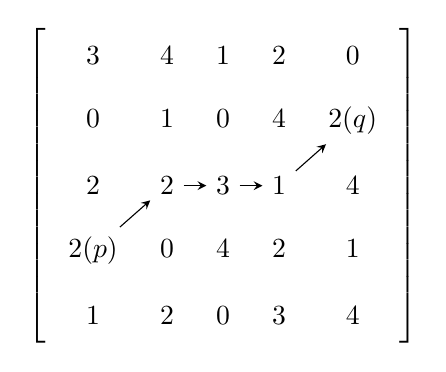
\begin{tikzpicture}
\matrix [matrix of math nodes,left delimiter={[},right delimiter={]}] (m)
{
    3 & [2ex] 4 & [2ex] 1 & [2ex] 2 & [2ex] 0\\[2ex]
    0 & [2ex] 1 & [2ex] 0 & [2ex] 4 & [2ex] 2(q)\\[2ex]
    2 & [2ex] 2 & [2ex] 3 & [2ex] 1 & [2ex] 4\\[2ex]
    2(p) & [2ex] 0 & [2ex] 4 & [2ex] 2 & [2ex] 1\\[2ex]
    1 & [2ex] 2 & [2ex] 0 & [2ex] 3 & [2ex] 4\\[2ex]
};
\path[-stealth] (m-4-1) edge (m-3-2);
\path[-stealth] (m-3-2) edge (m-3-3);
\path[-stealth] (m-3-3) edge (m-3-4);
\path[-stealth] (m-3-4) edge (m-2-5);
\end{tikzpicture}
\subcaption{Shortest 8-path}
\end{minipage}
\begin{minipage}[b]{0.45\linewidth}
\centering
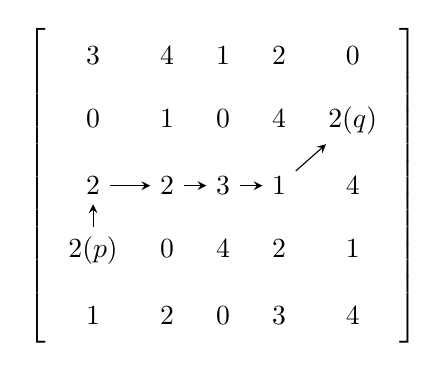
\begin{tikzpicture}
\matrix [matrix of math nodes,left delimiter={[},right delimiter={]}] (m)
{
    3 & [2ex] 4 & [2ex] 1 & [2ex] 2 & [2ex] 0\\[2ex]
    0 & [2ex] 1 & [2ex] 0 & [2ex] 4 & [2ex] 2(q)\\[2ex]
    2 & [2ex] 2 & [2ex] 3 & [2ex] 1 & [2ex] 4\\[2ex]
    2(p) & [2ex] 0 & [2ex] 4 & [2ex] 2 & [2ex] 1\\[2ex]
    1 & [2ex] 2 & [2ex] 0 & [2ex] 3 & [2ex] 4\\[2ex]
};
\path[-stealth] (m-4-1) edge (m-3-1);
\path[-stealth] (m-3-1) edge (m-3-2);
\path[-stealth] (m-3-2) edge (m-3-3);
\path[-stealth] (m-3-3) edge (m-3-4);
\path[-stealth] (m-3-4) edge (m-2-5);
\end{tikzpicture}
\subcaption{Shortest m-path}
\end{minipage}
\caption{Shortest paths}
\label{fig:adjacency}
\end{figure}

\subsection{Logical Operations}
\begin{enumerate}
\item $A \cap B \cap C$
\item $(A \cap B) \cup (B \cap C) \cup (A \cap C)$
\item $(\overline{A} \cap B \cap \overline{C}) \cup (A \cap \overline{B} \cap C)$
\end{enumerate}

\section{Programming Tasks}
\subsection{Scaling}

\subsubsection{Discussion}
\paragraph{}
There are~\ref{lastscale} common ways to scale a gray image \cite{leptonica}:

\begin{enumerate}
\item Sampling
\item Area mapping (or area averaging) and lowpass filtering
\item Mip-mapping
\item Min-max
\item Interpolation \label{lastscale}
\end{enumerate}

For this project, I used interpolation since it is available in many third-party libraries and can produce a good result.

\paragraph{}

There are~\ref{lastinterpolation} common interpolation methods \cite{gonzalez2008digital}:
\begin{enumerate}
\item Nearest-neighbor
\item Bilinear
\item Bicubic \label{lastinterpolation}
\end{enumerate}

I chose bicubic interpolation for this project because it is effcient enough, produces fewer interpolation artifacts, and is applicable for both down-scaling and up-scaling. The result are listed in section~\ref{sec:scaleresult}, and the algorithm is described in section~\ref{sec:scaleresult}. We can see that the false contouring starts to appear in the 32-level image.

\begin{description}
\item[Note] \hfill \\
Although I have not implement it, there is a very impressive image scaling algorithm, called \textit{seam carving} \cite{Avidan:2007:SCC:1275808.1276390}, which can scale an image to a new aspect ratio very natually.
\end{description}

\subsubsection{Results}
\label{sec:scaleresult}
\begin{figure}[H]
\centering
% pt = px * 72 / DPI
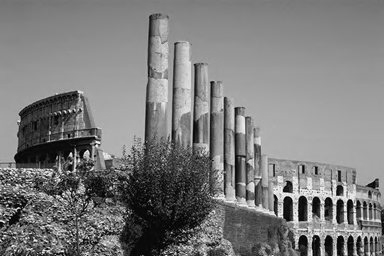
\includegraphics[width=288pt]{../img/02.png}
\caption{The original image}
\label{scaleorigin}
\end{figure}

\begin{figure}[H]
\centering
% pt = px * 72 / DPI
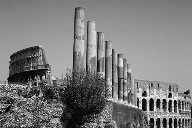
\includegraphics[width=144pt]{../result/scale-192-128.png}
\caption{Down-scale to $192 \times 128$}
\label{scale192}
\end{figure}

\begin{figure}[H]
\centering
% pt = px * 72 / DPI
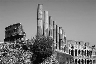
\includegraphics[width=72pt]{../result/scale-96-64.png}
\caption{Down-scale to $96 \times 64$}
\label{scale96}
\end{figure}

\begin{figure}[H]
\centering
% pt = px * 72 / DPI
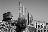
\includegraphics[width=36pt]{../result/scale-48-32.png}
\caption{Down-scale to $48 \times 32$}
\label{scale48}
\end{figure}

\begin{figure}[H]
\centering
% pt = px * 72 / DPI
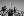
\includegraphics[width=18pt]{../result/scale-24-16.png}
\caption{Down-scale to $24 \times 16$}
\label{scale24}
\end{figure}

\begin{figure}[H]
\centering
% pt = px * 72 / DPI
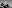
\includegraphics[width=9pt]{../result/scale-12-8.png}
\caption{Down-scale to $12 \times 8$}
\label{scale12}
\end{figure}

\begin{figure}[H]
\centering
% pt = px * 72 / DPI
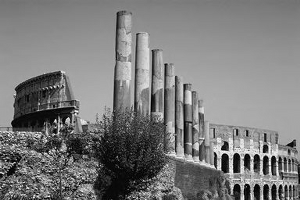
\includegraphics[width=225pt]{../result/scale-300-200.png}
\caption{Down-scale to $300 \times 200$}
\label{scale300}
\end{figure}

\begin{figure}[H]
\centering
% pt = px * 72 / DPI
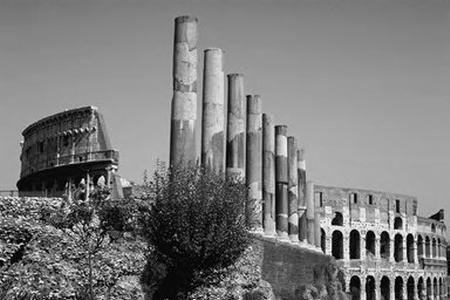
\includegraphics[width=337.5pt]{../result/scale-450-300.png}
\caption{Up-scale to $450 \times 300$}
\label{scale450}
\end{figure}

\begin{figure}[H]
\centering
% pt = px * 72 / DPI
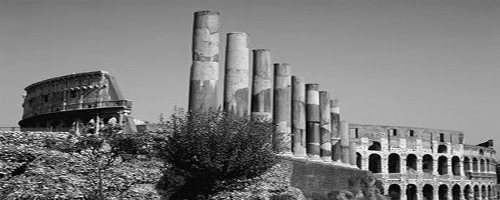
\includegraphics[width=375pt]{../result/scale-500-200.png}
\caption{Scale to $500 \times 200$}
\label{scale500}
\end{figure}

\subsubsection{Algorithm}
\label{sec:scalealgo}
\begin{algorithm}[H]
\centering
\caption{Scaling gray image}
\label{alg:scale}
  \begin{algorithmic}[1]
    \Function{Scale}{$input\_img$, $size$}
      \State Create an empty image $output\_img$ with $size$
	  \If{$input\_img.size$ == $size$}
        \State Copy $input\_img$ to $output\_img$
        \State \Return $output\_img$
	  \EndIf
      \State \textsc{Interpolate} $\gets$ \Call{GetInterpolation}{$input\_img$}
      \For{each pixel $(x, y)$ in $output\_img$}
      	\State $(relx, rely) \gets$ \Call{GetRelativePosition}{$x$, $y$, $size$, $input\_img.size$}
      	\State $new\_value \gets$ \Call{Interpolate}{$relx$, $rely$}
      	\State Put $new\_value$ back into $(x, y)$ in $output\_img$
      \EndFor
      \State \Return $output\_img$
    \EndFunction
    \\
    \Function{GetInterpolation}{$input\_img$}
      \State $x \gets [0, 1, ..., input\_img.width - 1]$
      \State $y \gets [0, 1, ..., input\_img.height - 1]$
      \For{each $j$ in $y$}
      	\For{each $i$ in $x$}
      	  \State $row \gets$ an empty list
      	  \State Append $input\_img.getpixel(i, j)$ to $row$
      	\EndFor
      	\State Append $row$ to $z$
      \EndFor
      \State \Return \Call{GetBicubicInterpolation}{$x$, $y$, $z$}
    \EndFunction
    \\
    \Function{GetRalativePosition}{$x$, $y$, $new\_size$, $old\_size$}
      \State $new\_width, new\_height = new\_size$
      \State $old\_width, old\_height = old\_size$
      \State $new\_x \gets x \times \frac{old\_width}{new\_width}$ 
      \State $new\_y \gets y \times \frac{old\_height}{new\_height}$ 
      \State \Return $new\_x, new\_y$
    \EndFunction
  \end{algorithmic}
\end{algorithm}

\subsection{Quantization}

\subsubsection{Discussion}

\paragraph{}
Although color quantization for a color image is complex, it is relatively simple to implement quantization for a gray image. For this project, I first compute the new palette for the given gray level, then replace each pixel with its nearest neighbor in this palette. This algorithm is somewhat similar to the median-cut algorithm applied in one dimension.

The results are listed in section~\ref{sec:quanresult}, and the algorithm is described in section~\ref{sec:quanalgo}.

\subsubsection{Results}
\label{sec:quanresult}
\begin{figure}[H]
\centering
% pt = px * 72 / DPI
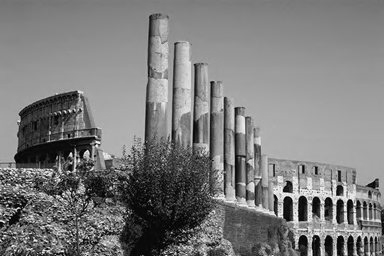
\includegraphics[width=288pt]{../img/02.png}
\caption{The original image}
\label{quanorigin}
\end{figure}

\begin{figure}[H]
\centering
% pt = px * 72 / DPI
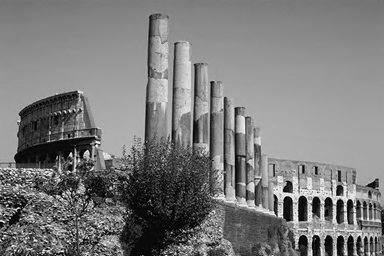
\includegraphics[width=288pt]{../result/quantize-128.png}
\caption{128 gray levels}
\label{quan128}
\end{figure}

\begin{figure}[H]
\centering
% pt = px * 72 / DPI
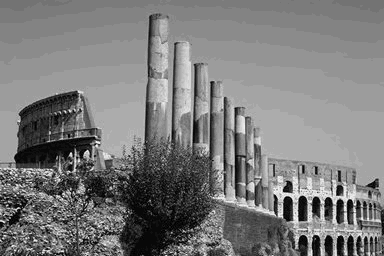
\includegraphics[width=288pt]{../result/quantize-32.png}
\caption{32 gray levels}
\label{quan32}
\end{figure}

\begin{figure}[H]
\centering
% pt = px * 72 / DPI
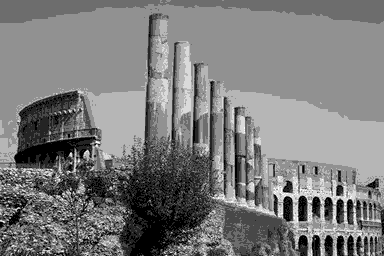
\includegraphics[width=288pt]{../result/quantize-8.png}
\caption{8 gray levels}
\label{quan8}
\end{figure}

\begin{figure}[H]
\centering
% pt = px * 72 / DPI
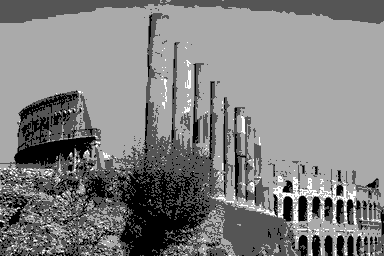
\includegraphics[width=288pt]{../result/quantize-4.png}
\caption{4 gray levels}
\label{quan4}
\end{figure}

\begin{figure}[H]
\centering
% pt = px * 72 / DPI
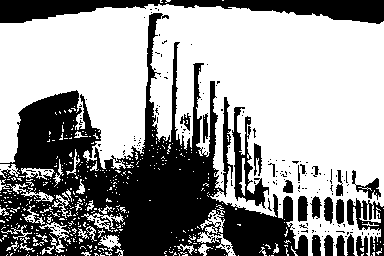
\includegraphics[width=288pt]{../result/quantize-2.png}
\caption{2 gray levels}
\label{quan2}
\end{figure}

\subsubsection{Algorithm}
\label{sec:quanalgo}
\begin{algorithm}[h]
\centering
\caption{Quantize gray image}
\label{alg:quan}
  \begin{algorithmic}[1]
    \Function{Quantize}{$input\_img, level$}
      \State Create an empty image $output\_img$ with $input\_img.size$
      \If{$input\_img.level$ == $level$}
      	\State Copy $input\_img$ to $output\_img$
      	\State \Return $output\_img$
      \EndIf
      \State $new\_pallete \gets [\lfloor255 \times \frac{i}{level-1}\rfloor$ for $i$ in $[0, 1, ..., level]$]
      \For{each pixel $(x, y)$ in $input_img$}
      	\State $new\_color \gets$ the nearest neighbor of the pixel color in $new\_pallete$
      	\State Put $new\_color$ into $(x, y)$ in the $output\_img$
      \EndFor
      \State \Return $output\_img$
    \EndFunction
  \end{algorithmic}
\end{algorithm}

\bibliography{scale}

\bibliographystyle{acm}

\end{document}